\documentclass[12pt]{article}
\usepackage{graphicx}
\usepackage[utf8]{inputenc}
\usepackage{relsize}
\usepackage{url}
\usepackage{color}
\usepackage{amsmath}
\usepackage{amssymb}
\usepackage{booktabs,caption}
\usepackage[flushleft]{threeparttable}
\begin{document}

a) 

\begin{table}[!htbp] \centering 
\begin{threeparttable}
  \caption{Pooling model regression results.} 
  \label{} 
\begin{tabular}{@{\extracolsep{5pt}}lcccc} 
 \toprule
\midrule
\\
Residuals: \\
\hline \\[-1.8ex] 
     Min. &  1st Qu.  &  Median &  3rd Qu.   &   Max. \\
-4.737340 & -0.606864 & 0.056466 & 0.727930 & 3.505346 \\
 & \\ 
Coefficients: \\
\hline \\[-1.8ex] 
       &       Estimate & Std. Error & t-value  & Pr($>|t|$)  \\
(Intercept) & -4.6742194  & 1.2981340 & -3.6007 & 0.0003515 *** \\
income    &   1.0357785  & 0.1289442  & 8.0328 & 7.935e-15 *** \\
price  &      0.4830921  & 0.2077034  & 2.3259 & 0.0204553 *  \\
age     &     1.5472745 & 0.2169547 & 7.1318 & 3.826e-12 *** \\
ms      &    -0.0080364  & 0.1848487 & -0.0435 & 0.9653411   \\
deps   &      0.1753681  & 0.0426421  & 4.1126 & 4.629e-05 *** \\
\bottomrule
 \end{tabular}
 \begin{tablenotes}
\small
\item \textit{Note:} Signif. codes:  0 ‘***’ 0.001 ‘**’ 0.01 ‘*’ 0.05 ‘.’ 0.1 ‘ ’ 1
\item \ 
\item Total Sum of Squares:    809.35 
\item Residual Sum of Squares: 627.66 
\item R-Squared:      0.22449 
\item Adj. R-Squared: 0.21613 
\item F-statistic: 26.8628 on 5 and 464 DF, p-value: $<$ 2.22e-16 
\end{tablenotes}
  \end{threeparttable}
\end{table} 

\newpage

\begin{table}[!htbp] \centering 
\begin{threeparttable}
  \caption{Individual fixed effects model regression results.} 
  \label{} 
\begin{tabular}{@{\extracolsep{5pt}}lcccc} 
 \toprule
\midrule
\\
Residuals: \\
\hline \\[-1.8ex]
     Min.  & 1st Qu. &   Median &  3rd Qu.   &   Max. \\
-3.608066 & -0.264850 &  0.030264  & 0.310411 &  2.348169 \\
\\
Coefficients: \\
\hline \\[-1.8ex] 
   &     Estimate & Std. Error &  t-value  & Pr($>|t|$)    \\
income &  0.838810  &  0.111267 & 7.5387 & 2.976e-13 *** \\
price  &  0.366080  &  0.124294 & 2.9453 &  0.003407 ** \\
age   &  0.102249  &  0.208039  & 0.4915 &  0.623338    \\
ms    &  0.199833 &  0.263890 & 0.7573  & 0.449322    \\
deps   & -0.086352  & 0.053483 & -1.6146 &  0.107154  \\
\bottomrule
 \end{tabular}
 \begin{tablenotes}  
\small
\item \textit{Note:} Signif. codes:  0 ‘***’ 0.001 ‘**’ 0.01 ‘*’ 0.05 ‘.’ 0.1 ‘ ’ 1
\item \ 
\item Total Sum of Squares:    221.58
\item Residual Sum of Squares: 191.67
\item R-Squared:      0.13497
\item Adj. R-Squared: 0.029433
\item F-statistic: 13.0445 on 5 and 418 DF, p-value: 8.2159e-12
\end{tablenotes}
  \end{threeparttable}
\end{table} 

\newpage

\begin{table}[!htbp] \centering 
\begin{threeparttable}
  \caption{Individual random effects model regression results.} 
  \label{} 
\begin{tabular}{@{\extracolsep{5pt}}lcccc} 
 \toprule
\midrule
\\
Residuals: \\
\hline \\[-1.8ex]
     Min.  & 1st Qu. &   Median &  3rd Qu.   &   Max. \\
-3.820238 & -0.278886 &  0.060427 &  0.371336 &  2.170378  \\
 \\
Coefficients:  \\
\hline \\[-1.8ex]
    &         Estimate Std. & Error & z-value & Pr($>|z|$)    \\ 
(Intercept) & -2.370567   & 1.114863 & -2.1263 &  0.033476 *   \\
income   &    0.852996  &  0.108734  & 7.8448 & 4.337e-15 *** \\
price    &    0.370199  &  0.125398  & 2.9522  & 0.003155 **  \\
age     &     0.277063  &  0.201695  & 1.3737  & 0.169544     \\
ms      &     0.199669  &  0.233954 &  0.8535  & 0.393406     \\
deps   &     -0.036254 & 0.049289 & -0.7355 & 0.462013   \\
\bottomrule
 \end{tabular}
 \begin{tablenotes}    
\small
\item \textit{Note:} Signif. codes:  0 ‘***’ 0.001 ‘**’ 0.01 ‘*’ 0.05 ‘.’ 0.1 ‘ ’ 1
\item \ 
\item Total Sum of Squares:    251.12
\item Residual Sum of Squares: 217.79
\item R-Squared:      0.1327
\item Adj. R-Squared: 0.12335
\item Chisq: 70.9941 on 5 DF, p-value: 6.3636e-14
\end{tablenotes}
  \end{threeparttable}
\end{table} 


c)

\begin{table}[!htbp] \centering 
\begin{threeparttable}
  \caption{Oneway (individual) effect Random Effect Model (Swamy-Arora's transformation).} 
  \label{} 
\begin{tabular}{@{\extracolsep{5pt}}lcccc} 
 \toprule
\midrule
\\
Effects: \\
\hline \\[-1.8ex]
      &           var & std.dev & share & \\
$\hat\sigma_\epsilon^2$ (idiosyncratic): & 0.4585 &  0.6772 & 0.346 & \\
$\hat\sigma_v^2$ (individual):  &  0.8666 & 0.9309 & 0.654 & \\
\\
$\theta$: & 0.7758 & &  & \\
\bottomrule
 \end{tabular}
 \begin{tablenotes}    
\small
\item \textit{Notes:} 
\item
\item plm(formula = charity ~ income + price + age + ms 
\item + deps, data = df, model = "random")
\item
\item Balanced Panel: n = 47, T = 10, N = 470
\end{tablenotes}
  \end{threeparttable}
\end{table} 


\newpage

d)
\begin{flushleft}
F(5, 464) = 26.8628 $>$ 1.14
\break
F(5, 464) critical value is equal to 1.14 using a 5\% level of significance.
\end{flushleft}

e) **********
\begin{flushleft}
Breusch-Pagan test for heteroskedasticity (in gretl) -
\break
Null hypothesis: heteroskedasticity not present
\break
Test statistic: LM = 32.2872
\break
with p-value = P(Chi-square(5) $>$ 32.2872) = 5.21172e-06
\end{flushleft}

f) **********
\begin{flushleft}
Hausman Test (in R):
\break
data:  charity $\sim$ income + price + age + ms + deps
\break
chisq = 19.245, df = 5, p-value = 0.00173
\break
alternative hypothesis: one model is inconsistent
\end{flushleft}

\newpage

l) (Arelland-Bond linear dynamic panel)

\begin{figure}[h!]
\begin{center}
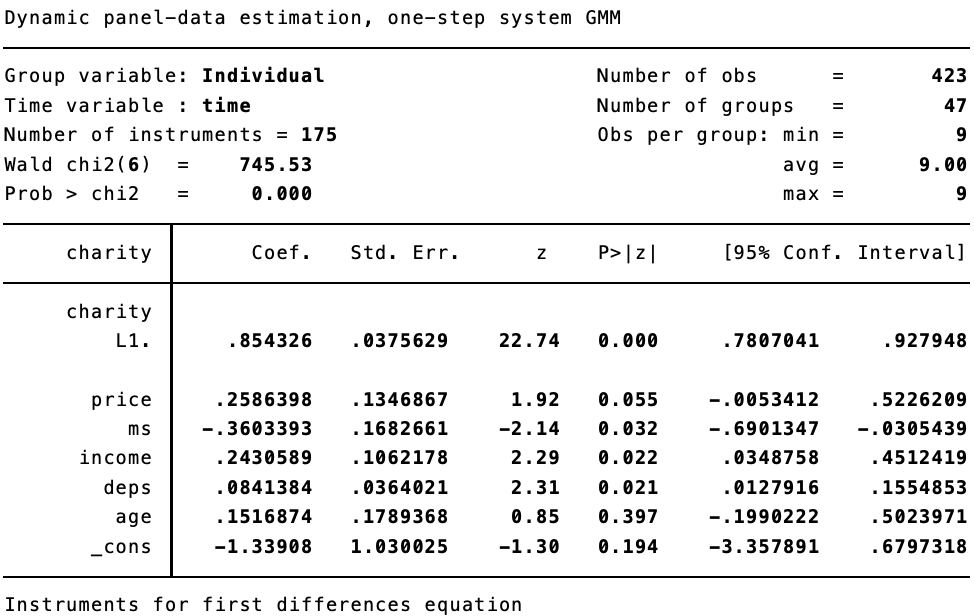
\includegraphics[scale=0.85]{GMM.png}
\label{}
\caption{Arelland-Bond GMM regression results.}
\end{center}
\end{figure}



\end{document}